\subsection{CapTap}
\label{ch:prot_captap}
\begin{figure}[h]
\centering
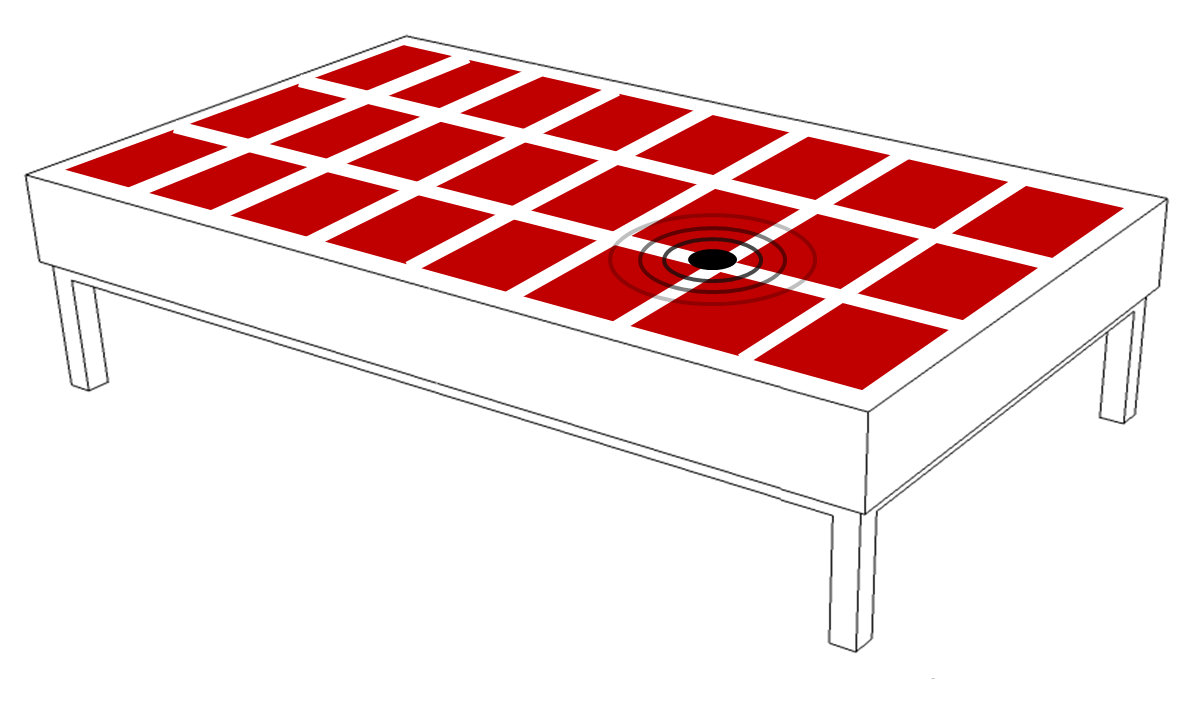
\includegraphics[width=0.7\textwidth]{images/captap_v2}
\caption{CapTap sketch - 24 electrodes placed under table surface and a single detector for touch events}
\label{fig:captap_sketch}
\end{figure}
A general insight of free-air gestural interaction that became apparent even in early works is the physical demands of prolonged interaction with such systems \cite{Baudel1993, lenman2002} and the difficulty to adapt selection events to gestural input - the latter typically being realized by time- or position-based gestures \cite{Baudel1993,Krum2002}. There is no trivial solution to this challenge and any approach has to take into account the specific application scenario covered. Some systems attempt to provide specifically adapted graphical interfaces, while others include additional input devices assisting the interaction \cite{Wu2003,zimmerman1987hand}. A major point is decreasing the required time for interaction, e.g. by adding a tactile feedback to the interaction system, preventing time-based selection gestures. CapTap is a regular living room table that includes a capacitive proximity sensor array for tracking the position of one or more arms. As it is difficult for this sensor category to detect touch, if the interaction surface is at a distance from the electrodes, a hidden acoustic system is added that allows recognizing different touch events. CapTap tracks hand and arm position using the image-based object recognition previously presented and fuses this data with different touch events generated by a single contact microphone that analyzes the audio signals in frequency space. This allows to significantly reduce interaction time, as opposed to systems relying on time-based dwell gestures. The system was created in 2013 and 2014 with collaboration of several students, most notably Sebastian Zander-Walz and Stefan Frank \cite{Braun2013captap}. It is used and further developed within the European research project POSEIDON that aims at providing technical solutions to help persons with Down's syndrome on planning their day. The idea is to have an input device that allows interaction regardless of motoric skill level.
\subsubsection{Capacitive layout}
\begin{figure}[ht]
\centering
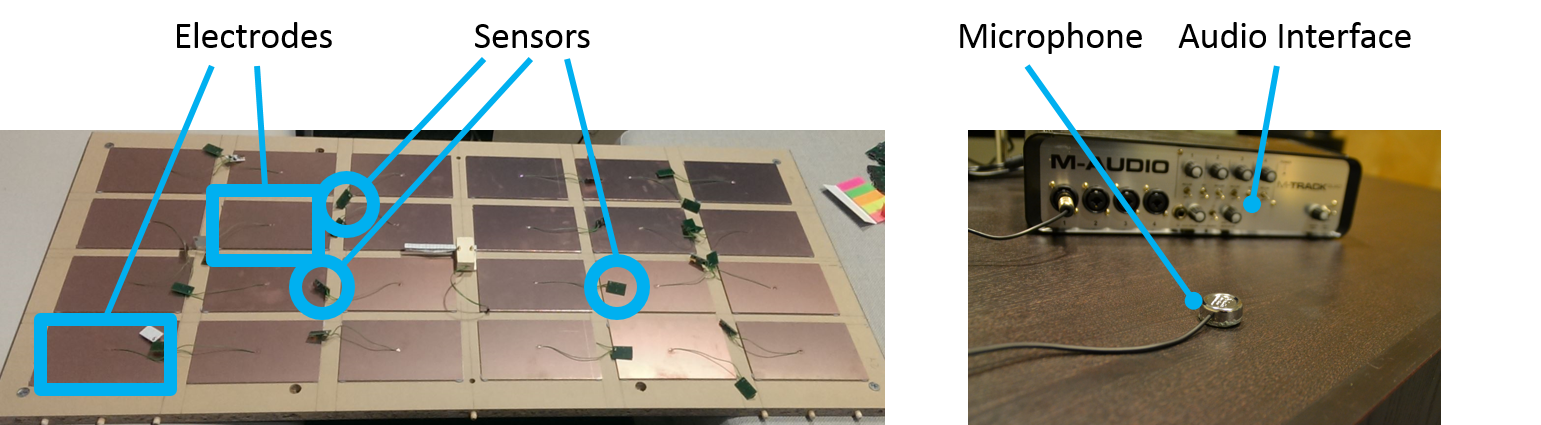
\includegraphics[width=0.8\textwidth]{images/prototype_views_new}
\caption{Detail views of the prototype system: left - electrodes and sensors, right - audio interface and contact microphone}
\label{fig:prototype_views_new}
\end{figure}	
 
Our goal with CapTap is to enable tracking of hands and arms that move above a table. Therefore, the electrodes are placed in an uniform array that provides similar sensing properties for the whole surface. It is realized as a prototype installed in a regular living room table. It is comprised of an array of capacitive proximity sensors, a contact microphone for touch event detection and a miniature PC. All devices can be integrated into the table in a way that it is not distinguishable from the not-augmented piece of furniture. Figure \ref{fig:prototype_views_new} shows some detail views of the disassembled prototype. The left image shows the back of the wooden tabletop. The electrodes are arranged in a 6x4 array and each one is attached to a single sensor. The right picture shows the touch detection microphone. It is attached in the center of the surface, as to avoid non-uniform sound distribution over the surface area that would be more difficult to train. Placing the microphone below the surface has no strong influence. However, a specific training phase is required for any novel surface that is equipped with the touch detection devices. 

\begin{figure}[ht]
\centering
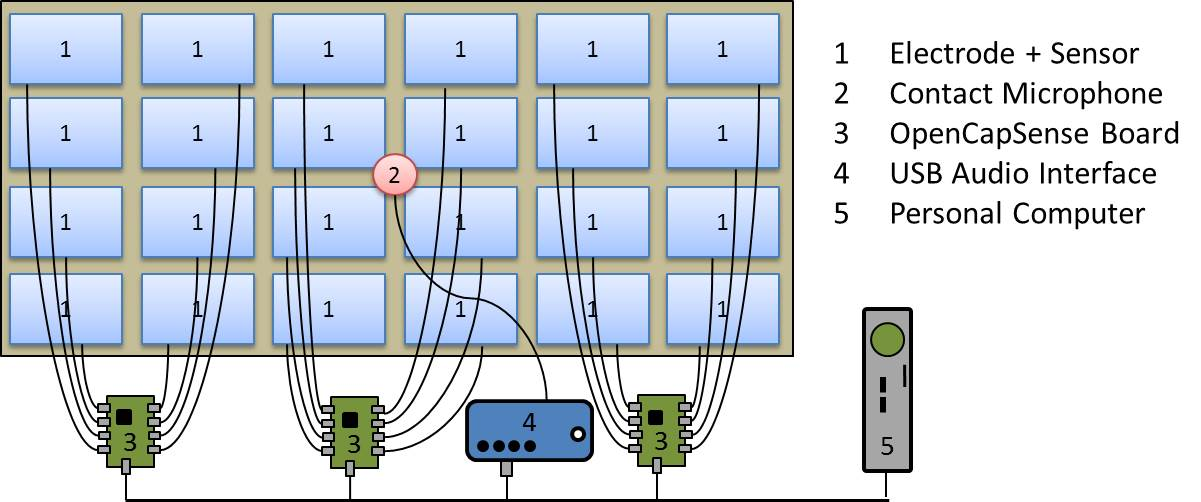
\includegraphics[width=0.8\textwidth]{images/captap_schematics}
\caption{Abstract view below the surface of the prototype including capacitive sensing electrodes and touch detection microphone}
\label{fig:captap_schematics}
\end{figure}

The setup is visualized in Figure \ref{fig:captap_schematics}. The system is comprised of 24 electrode \& sensor pairs that are connected to three different measurement boards. The microphone is attached to a USB Audio Interface. Overall there are four different boards connected via USB to a  PC that executes and merges the different types of data processing and links it to the software suite. The prototype is based on OpenCapSense, a more advanced prototyping system presented by Grosse-Puppendahl et al. \cite{grosse2013opencapsense}. The boards are performing some prefiltering, whereas the image-based hand tracking is realized on an attached PC. The microphone is attached to an USB audio interface (M-Audio M-Track Quad) that transfers data acquired by up to four microphones and provides various pre-sampling functions. All four devices are attached to a Mini-PC that is performing subsequent data processing and is running the demonstration and testing applications. 
 
\begin{figure}[ht]
\centering
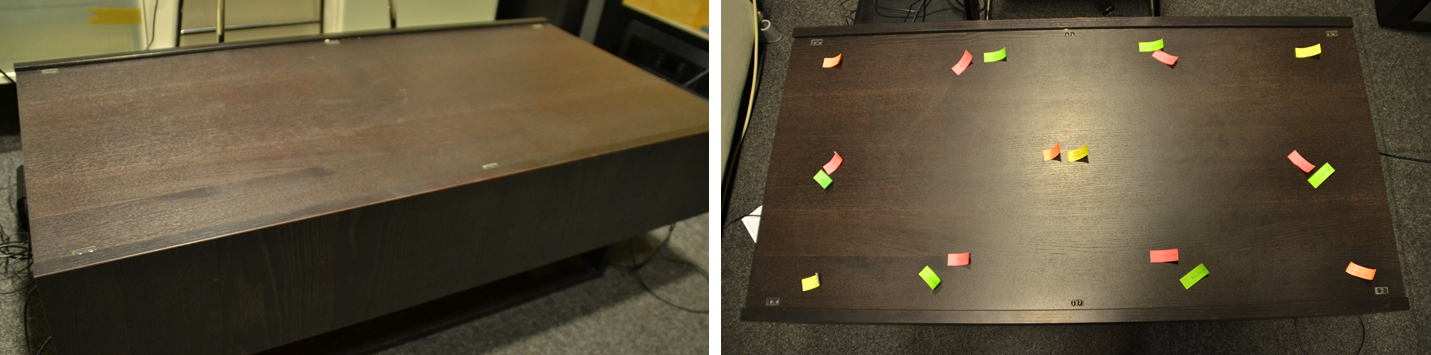
\includegraphics[width=0.8\textwidth]{images/table_final_view}
\caption{Views of final prototype, complete view (left), top view with markers for touch evaluation (right)}
\label{fig:table_final_view}
\end{figure}

The final table prototype can be seen in Figure \ref{fig:table_final_view}. On the left side the table is seen without any additional markers - on the right side we see the table equipped for the evaluation using a set of markers for different touch and swipe events. The debug software was developed with C\# using the .NET 4.5 framework. We are using the Emgu CV library based on OpenCV for image processing and application of the Kalman filter to the determined palm locations. The sound processing is implemented in C++ and Java using a modified version of ChucK for audio sampling and the WEKA framework to apply the machine learning on top. We are using sockets to transfer data between the different modules. The debug application allows a fine control of the various processing steps in both image and audio signal processing.

\subsubsection{Processing}
CapTap is using the image-based algorithm for tracking palms and arms that was presented in Section \ref{ch:proc_image}. An addition is the touch recognition based on acoustic tracking. The method was inspired by the works of Harrison et al. \cite{harrison2011tapsense} with various modifications to allow identifying both impact and swipe events. At first the audio signal is acquired using a 96kHz sample rate and a feature extraction rate of 375Hz (using a  Hanning type sliding window of 4096 (and 256 samples overlapping) samples per extraction. In order to perform a classification over this signal we have to look at a variety of different features.

The signal differences are most significant in the frequency domain, thus we are performing a FFT over 4096 samples, looking at the first 512 of 2048 magnitude values, thus covering the frequency range up to 12kHz. We are collecting the mean value, the standard deviation and the index of the highest value within the frequency range. This process is repeated for a downsampled FFT of 64 values, similar to the method used by Harrison et al. Another frequency domain-feature we are using is the centroid, i.e. the weighted mean of the present frequencies. Additionally, we are using two time-domain features, the RMS power (root mean square), i.e. the average magnitude within the current frequency band and the number of zero crossings of the signal. 

We have to distinguish two different classifiers that are used for impact and swiping events. Even though knocks and taps are temporal gestures they are short in duration, while the swipe gestures are constant for a longer time period. Example 64-value FFTs are shown in Figure \ref{fig:alltouch}, with impact events and their low-frequency peaks on the left and swipe events and their fairly constant value on the right. For impact events we are using some metrics to identify the point at which the features shall be analyzed. A simple preprocessing identifies increasing power in lower frequencies and begins to store all feature vectors until a maximum is reached or the power is decreasing again. Not relevant secondary power increases (that are prevalent on stronger knocking events) are ignored. The feature vector corresponding to the maximum is then put into the classifier. This is a trained SMO classifier comprised of a support vector machine and a polynomial kernel that matches five different impacts - single knock, double knock, single finger tap, single double tap, and stomps that are classified but not used any further.
The classification of different swipe events is realized using a sliding window over a set of previous feature vectors. The derived feature set is comprised primarily of average and standard deviations of the single items within the previous feature vectors. The FFT values are most relevant. This combined feature set is fed into a decision tree that is using several thresholds to decide if the swipe was performed by a finger or the whole hand. We are using the effect that swipes have fairly constant values in the frequency band between 2kHz and 8kHz. This classification is performed each 256 samples. In order for a swipe gesture to be identified a number of subsequent positive classifications have to occur. For example 10 classifications that indicate a constant movement of 26ms or more are identified as a swipe gesture.

\subsubsection{Evaluation}
In order to evaluate our system we have performed a combined study by 10 users who were invited to test the accuracy of the touch detection and benchmark the interaction speed. They predominantly had plenty of experience with touch devices (all questionnaire questions refer to Likert-scale 1 to 10, $\mu=9.40, \sigma=1.90$). Experience with gesture interaction systems like the Kinect or Leap Motion was less prevalent and had a higher variation ($\mu=6.00, \sigma=2.71$).
 
\begin{figure}[ht]
\centering
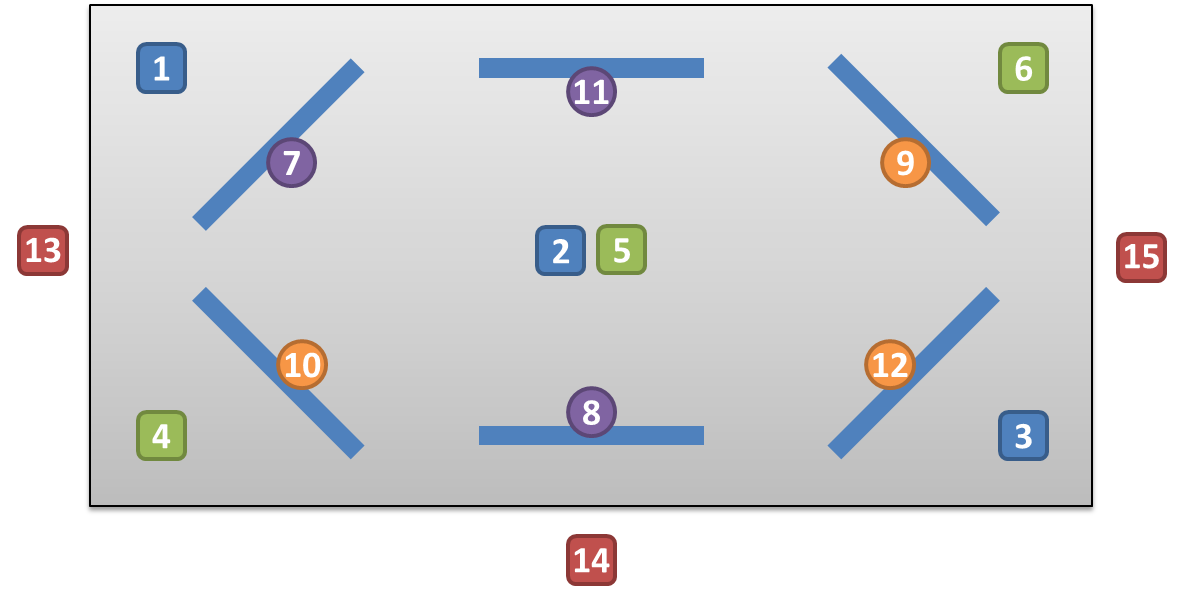
\includegraphics[width=0.8\textwidth]{images/eval_touch_v2}
\caption{Finger tap (blue), knuckle knock (green), finger swipe (purple), hand swipe (orange) and stomping (red) spots relative to tabletop.}
\label{fig:eval_touch_v2}
\end{figure}

\subsubsection*{Touch detection accuracy}
One of the main interesting aspects for us is the accuracy of the touch detection with a classification that is only trained by a limited number of users. Six different types of touch events are tested by the different users - finger tap, double finger tap, knuckle knock, double knuckle knock, finger swipe and hand swipe. In addition we want to get an idea if outside influences can disturb the signal, thus we are letting the users stomp at three different locations in close proximity of the table. Overall we have 12 different areas on the table that have to be touched in different ways by the users. These are executed three times each, leading to 54 touch samples and 9 stomp samples. The locations shown in Figure \ref{fig:eval_touch_v2} are (double) finger taps (1,2,3), (double) knuckle knocks (4,5,6), finger swipes (7,8,9), hand swipes (10,11,12) and  stomps (13,14,15). The main purpose of this evaluation was to test a pre-trained algorithm that does not require any training efforts by the user. The subjects were shown all different supported touch gestures just once in a live example. The results are shown in Table \ref{tab:prot_captap_eval_knock}. The system was very well capable of recognizing the different taps having a success rate of 96\% or more. The results were not as good for knock detection, with only 81\% correct classification of single knocks and 60\% correct classification of double knocks. However, it should be noted that there was a high variance in results.
 
\begin{table}[htbp]
  \centering
  \caption{Results of touch detection for single and double taps (SFT, DFT), knocks (SKK, DKK), finger swipe (FS), hand swipe (HS) and stomp (STO). Noted are the overall samples, errors, no event errors, wrong classification errors and the percentage of correct classification.}
    \begin{tabular}{lccccccc}
    \toprule
          & \textbf{SFT} & \textbf{DFT} & \textbf{SKK} & \textbf{DKK} & \textbf{FS} & \textbf{HS} & \textbf{STO} \\
    \midrule
    \textbf{Samples} & 90    & 90    & 90    & 90    & 90    & 90    & 90 \\
    \textbf{Errors} & 1     & 3     & 17    & 36    & 18    & 2     & 22 \\
    \textbf{No event} & 1     & 0     & 0     & 0     & 6     & 0     & 0 \\
    \textbf{Wrong Class} & 0     & 3     & 17    & 36    & 12    & 2     & 22 \\
    \textbf{Percentage correct class} & 98,89 & 96,67 & 81,11 & 60    & 80    & 97,78 & 75,56 \\
    \bottomrule
    \end{tabular}%
  \label{tab:prot_captap_eval_knock}%
\end{table}%

Two users accounted for half the errors of double knock recognition as none of their double knocks were recognized. Thus with some additional training and adaptation it should be possible to detect all knocks. The classification of finger swipes showed similar results. The majority of errors (15 of 18) were produced by a small set of subjets (3 of 10), leading to a detection rate of only 80\%. Again, training the different gestures should lead to an improvement. The results for hand swipe were very favorable with a detection rate of almost 98\%. Stomps were able to disturb the system in about 25\% of all events. However, in practical applications they are not highly relevant, as we can rule out any events where no hand is present above the table. Our tests showed that it is also very important to consider the uniformity of the table. The recognition rate of finger swipes at position 8 (93.33\%) was considerable better than the recognition at positions 7 and 9 (73.33\% for both), indicating that it is important to test each touch gesture at various positions and adjust the algorithm accordingly.
\subsubsection*{Hand tracking and interaction speed}

\begin{figure}[ht]
\centering
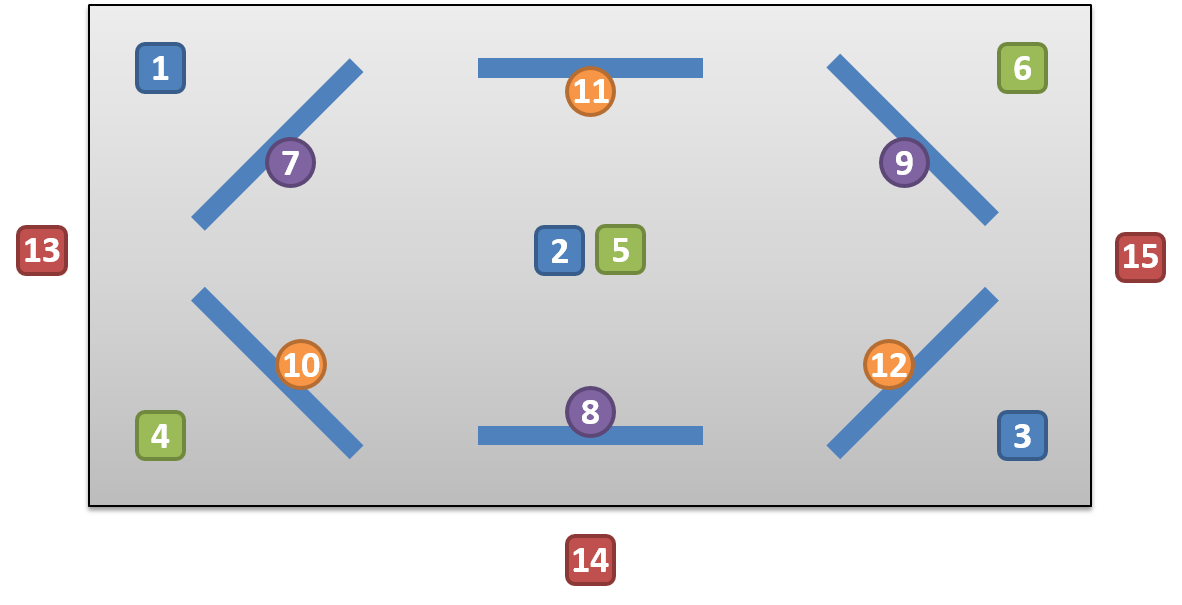
\includegraphics[width=0.8\textwidth]{images/knock_points}
\caption{Tracks generated by Kalman filtered palm position, a sine wave (A), a rectangle (B), a circle (C), and a diagonal swipe (D)}
\label{fig:tracks}
\end{figure}

In order to properly identify gestures the recognized paths of the hands are the most important measure. We have added a visualization module to the registered camera image introduced previously that allows us to show the tracks followed by one or more hands. Figure \ref{fig:tracks} shows several of the paths that were generated this way using single hand tracking. The hand is in this case moving about 10-15 cm above the table surface. While we have not connected the system to a generic path-based gesture recognition system, we can see that the system can create smooth trajectories that can be analyzed further.

A major point of interest for us was to check if users could successfully use the layer interaction pattern introduced before and if the option for adding unobtrusive touch detection would have any influence on the interaction speed. For this we used a small game whereas the participants had to put a cursor into a box and perform either a dwell (approximately 300ms) or touch activity for selection. The cursor reflected the current interaction layer by color coding. We counted the time it took to complete a run of 15 boxes.

\begin{figure}[ht]
\centering
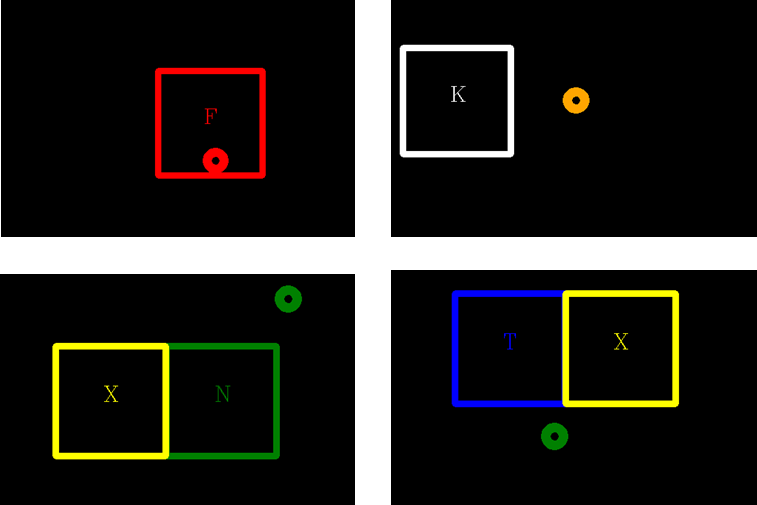
\includegraphics[width=0.7\textwidth]{images/eval_speed}
\caption{Interaction speed evaluation. Different types of boxes for near layer (N), knock (K), far layer (F), and disturber (X).}
\label{fig:eval_speed}
\end{figure}

Some example boxes are shown in Figure \ref{fig:eval_speed}. There were six different types referring to dwelling in the three different layers, knock, tap and disturber. Each participant performed four runs. First a training run, then a run with all interaction layers and the two touch events, then a run with dwelling boxes only (without layers), and finally a run with tap boxes only. The dwell and tap runs also included some disturber boxes to slightly increase the challenge. The order of the runs were switched equally between the different participants. Regarding the full interaction run we wanted to know if the user understands the different layers and can achieve a good interaction speed. The main hypothesis we wanted to test was that tapping improves the interaction speed as opposed to dwelling and may reduce the overall interaction times, thus reducing potential fatigue. We expected the tap run to be shorter than the dwell run as selection events can be performed faster. All runs had the same overall distance and the last two had inverse order to account for Fitts’ law.

\begin{table}[htbp]
  \centering
  \caption{Results for interaction time in the different runs of the interaction speed test}
    \begin{tabular}{lccc}
    \toprule
          & \textbf{Full run} & \textbf{Dwell run} & \textbf{Tap run} \\
    \midrule
    \textbf{Average Time} & 40.12 & 37.97 & 33.42 \\
    \textbf{Shortest Run} & 27.28 & 32.20 & 24.29 \\
    \textbf{Longest Run} & 51.38 & 48.11 & 47.72 \\
    \textbf{Standard Deviation} & 7.22 & 5.27 & 7.93 \\
    \bottomrule
    \end{tabular}%
  \label{tab:prot_captap_eval_intspeed}%
\end{table}%

The results are shown in Table \ref{tab:prot_captap_eval_intspeed}. Running a paired t-test on dwell and tap run the resulting p value is 0.0071, indicating a high statistical significance that the interaction using taps is faster than the interaction using dwelling. This fits expectations from literature \cite{lenman2002}. While this can be countered by reducing the dwell time, the risk of wrongful selection of nearby objects increases significantly.

Finally, we asked all participants to fill in a questionnaire with Likert-style questions in the style mentioned at the beginning of this section. Most users considered the device to be easy and precise enough to use ($\mu=8.1, \sigma=1.52$) and considered it highly intuitive ($\mu=8.9, \sigma=0.74$). Regarding the layer model they had no problem using it in the full test run ($\mu=8.6, \sigma=0.97$) but were critical to adding more layers ($\mu=3.9, \sigma=2.08$). They clearly preferred ($\mu=2.6, \sigma=2.72$) finger taps (Likert score 1) to knocks (Likert score 10). There was no clear preference for finger swipes (score 1) or hand swipes (score 10) ($\mu=4.6, \sigma=3.06$). The participants considered CapTap to be an interesting interaction device ($\mu=9.1, \sigma=1.20$) and could even imagine using it for longer periods ($\mu=6.9, \sigma=1.97$). Asking for particular points that they liked about the current version of CapTap the comments mentioned the ease of use and the high variety of different input commands that are supported. Points that were disliked are the usage of knocks that were considered unpleasant after a short while, even during the 10 minute study that only included few knocks. The hand tracking at this point is sometimes disturbed by the user's knees that enter the generated electric field around the table.


